\documentclass{standalone}
\usepackage{tikz}
\usetikzlibrary{calc, shapes, patterns, decorations.pathreplacing}

\begin{document}
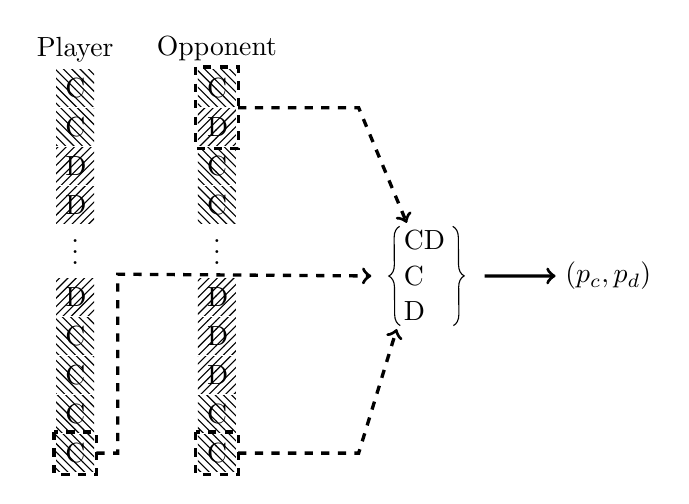
\begin{tikzpicture}[scale=.9]
    \tikzstyle{cooperator} = [rectangle, pattern=north west lines, text width=.25cm]
    \tikzstyle{defector} = [rectangle, pattern=north east lines, text width=.25cm]


    % Histories ----------------------------------------
    \node (A) at (-.5, 0) {Player};
    \node (A1) at ($(A) + (0, -.55)$) [cooperator] {C};
    \node (A2) at ($(A1) + (0, -.55)$) [cooperator] {C};
    \node (A3) at ($(A2) + (0, -.55)$) [defector] {D};
    \node (A4) at ($(A3) + (0, -.55)$) [defector] {D};
    \node (A5) at ($(A4) + (0, -.55)$) {$\vdots$};
    \node (A6) at ($(A5) + (0, -.75)$) [defector] {D};
    \node (A7) at ($(A6) + (0, -.55)$) [cooperator] {C};
    \node (A8) at ($(A7) + (0, -.55)$) [cooperator] {C};
    \node (A9) at ($(A8) + (0, -.55)$) [cooperator] {C};
    \node (A10) at ($(A9) + (0, -.55)$) [cooperator] {C};


    \node (B) at ($(A) + (2, 0)$) {Opponent};
    \node (B1) at ($(B) + (0, -.55)$) [cooperator] {C};
    \node (B2) at ($(B1) + (0, -.55)$) [defector] {D};
    \node (B3) at ($(B2) + (0, -.55)$) [cooperator] {C};
    \node (B4) at ($(B3) + (0, -.55)$) [cooperator] {C};
    \node (B5) at ($(B4) + (0, -.55)$) {$\vdots$};
    \node (B6) at ($(B5) + (0, -.75)$) [defector] {D};
    \node (B7) at ($(B6) + (0, -.55)$) [defector] {D};
    \node (B8) at ($(B7) + (0, -.55)$) [defector] {D};
    \node (B9) at ($(B8) + (0, -.55)$) [cooperator] {C};
    \node (B10) at ($(B9) + (0, -.55)$) [cooperator] {C};
    % ---------------------------------------------------

    % % Identifying inputs --------------------------------
    \draw[very thick, black, dashed] ($(B1) + (-.3, .3)$)  rectangle ($(B2) + (.3, -.3)$);
    \draw[very thick, black, dashed] ($(A10) + (-.3, .3)$)  rectangle ($(A10) + (.3, -.3)$);
    \draw[very thick, black, dashed] ($(B10) + (-.3, .3)$)  rectangle ($(B10) + (.3, -.3)$);

    % Strategy inputs
    \node (opp_start) at (4, -2.7) [right] {CD};
    \node (player_history) at (4, -3.2) [right] {C};
    \node (opp_history) at (4, -3.7) [right] {D};

    \draw [very thick, black, dashed, ->] ($(B1)!0.5!(B2) + (.3, 0)$) --
        ($(B1)!0.5!(B2) + (2, 0)$) -- ($(opp_start) + (-.25, .25)$);
    \draw [very thick, black, dashed, ->] ($(A10)!0.5!(A10) + (.3, 0)$) --
        ($(A10)!0.5!(A10) + (.6, 0)$) -- ($(A7)!0.5!(A10) + (.6, 1.7)$) --
        ($(player_history) + (-.6, 0)$);
    \draw [very thick, black, dashed, ->] ($(B10)!0.5!(B10) + (.3, 0)$) --
        ($(B10)!0.5!(B10) + (2, 0)$) -- ($(opp_history) + (-.25, -.25)$);

    % % Strategy outputs

    \draw [decorate, decoration={brace, amplitude=4pt}] ($(opp_start) + (.4, .2)$) --
    ($(opp_history) + (.55, -.2)$);

    \draw [decorate, decoration={brace, amplitude=4pt, mirror}] ($(opp_start) + (-.35, .2)$) --
    ($(opp_history) + (-.20, -.2)$);

    \node (output) at ($(player_history) + (2, 0)$) [right] {\((p_c, p_d)\)};

    \draw [->, very thick] ($(player_history) + (1, 0)$) -- (output);
\end{tikzpicture}
\end{document}
